\documentclass[twoside]{book}

% Packages required by doxygen
\usepackage{fixltx2e}
\usepackage{calc}
\usepackage{doxygen}
\usepackage[export]{adjustbox} % also loads graphicx
\usepackage{graphicx}
\usepackage[utf8]{inputenc}
\usepackage{makeidx}
\usepackage{multicol}
\usepackage{multirow}
\PassOptionsToPackage{warn}{textcomp}
\usepackage{textcomp}
\usepackage[nointegrals]{wasysym}
\usepackage[table]{xcolor}

% Font selection
\usepackage[T1]{fontenc}
\usepackage[scaled=.90]{helvet}
\usepackage{courier}
\usepackage{amssymb}
\usepackage{sectsty}
\renewcommand{\familydefault}{\sfdefault}
\allsectionsfont{%
  \fontseries{bc}\selectfont%
  \color{darkgray}%
}
\renewcommand{\DoxyLabelFont}{%
  \fontseries{bc}\selectfont%
  \color{darkgray}%
}
\newcommand{\+}{\discretionary{\mbox{\scriptsize$\hookleftarrow$}}{}{}}

% Page & text layout
\usepackage{geometry}
\geometry{%
  a4paper,%
  top=2.5cm,%
  bottom=2.5cm,%
  left=2.5cm,%
  right=2.5cm%
}
\tolerance=750
\hfuzz=15pt
\hbadness=750
\setlength{\emergencystretch}{15pt}
\setlength{\parindent}{0cm}
\setlength{\parskip}{3ex plus 2ex minus 2ex}
\makeatletter
\renewcommand{\paragraph}{%
  \@startsection{paragraph}{4}{0ex}{-1.0ex}{1.0ex}{%
    \normalfont\normalsize\bfseries\SS@parafont%
  }%
}
\renewcommand{\subparagraph}{%
  \@startsection{subparagraph}{5}{0ex}{-1.0ex}{1.0ex}{%
    \normalfont\normalsize\bfseries\SS@subparafont%
  }%
}
\makeatother

% Headers & footers
\usepackage{fancyhdr}
\pagestyle{fancyplain}
\fancyhead[LE]{\fancyplain{}{\bfseries\thepage}}
\fancyhead[CE]{\fancyplain{}{}}
\fancyhead[RE]{\fancyplain{}{\bfseries\leftmark}}
\fancyhead[LO]{\fancyplain{}{\bfseries\rightmark}}
\fancyhead[CO]{\fancyplain{}{}}
\fancyhead[RO]{\fancyplain{}{\bfseries\thepage}}
\fancyfoot[LE]{\fancyplain{}{}}
\fancyfoot[CE]{\fancyplain{}{}}
\fancyfoot[RE]{\fancyplain{}{\bfseries\scriptsize Generated by Doxygen }}
\fancyfoot[LO]{\fancyplain{}{\bfseries\scriptsize Generated by Doxygen }}
\fancyfoot[CO]{\fancyplain{}{}}
\fancyfoot[RO]{\fancyplain{}{}}
\renewcommand{\footrulewidth}{0.4pt}
\renewcommand{\chaptermark}[1]{%
  \markboth{#1}{}%
}
\renewcommand{\sectionmark}[1]{%
  \markright{\thesection\ #1}%
}

% Indices & bibliography
\usepackage{natbib}
\usepackage[titles]{tocloft}
\setcounter{tocdepth}{3}
\setcounter{secnumdepth}{5}
\makeindex

% Hyperlinks (required, but should be loaded last)
\usepackage{ifpdf}
\ifpdf
  \usepackage[pdftex,pagebackref=true]{hyperref}
\else
  \usepackage[ps2pdf,pagebackref=true]{hyperref}
\fi
\hypersetup{%
  colorlinks=true,%
  linkcolor=blue,%
  citecolor=blue,%
  unicode%
}

% Custom commands
\newcommand{\clearemptydoublepage}{%
  \newpage{\pagestyle{empty}\cleardoublepage}%
}

\usepackage{caption}
\captionsetup{labelsep=space,justification=centering,font={bf},singlelinecheck=off,skip=4pt,position=top}

%===== C O N T E N T S =====

\begin{document}

% Titlepage & ToC
\hypersetup{pageanchor=false,
             bookmarksnumbered=true,
             pdfencoding=unicode
            }
\pagenumbering{alph}
\begin{titlepage}
\vspace*{7cm}
\begin{center}%
{\Large The Rooms of L\textquotesingle{}ern -\/ Match2 \\[1ex]\large 1.\+0 }\\
\vspace*{1cm}
{\large Generated by Doxygen 1.8.14}\\
\end{center}
\end{titlepage}
\clearemptydoublepage
\pagenumbering{roman}
\tableofcontents
\clearemptydoublepage
\pagenumbering{arabic}
\hypersetup{pageanchor=true}

%--- Begin generated contents ---
\chapter{Hierarchical Index}
\section{Class Hierarchy}
This inheritance list is sorted roughly, but not completely, alphabetically\+:\begin{DoxyCompactList}
\item Application\begin{DoxyCompactList}
\item \contentsline{section}{G\+U\+I\+Match}{\pageref{class_g_u_i_match}}{}
\end{DoxyCompactList}
\item Event\+Handler\begin{DoxyCompactList}
\item \contentsline{section}{G\+U\+I\+Match.\+My\+Key\+Handler}{\pageref{class_g_u_i_match_1_1_my_key_handler}}{}
\end{DoxyCompactList}
\item \contentsline{section}{Match\+Grid}{\pageref{class_match_grid}}{}
\item Stack\+Pane\begin{DoxyCompactList}
\item \contentsline{section}{Match\+Tile}{\pageref{class_match_tile}}{}
\end{DoxyCompactList}
\end{DoxyCompactList}

\chapter{Class Index}
\section{Class List}
Here are the classes, structs, unions and interfaces with brief descriptions\+:\begin{DoxyCompactList}
\item\contentsline{section}{\mbox{\hyperlink{class_g_u_i_match}{G\+U\+I\+Match}} }{\pageref{class_g_u_i_match}}{}
\item\contentsline{section}{\mbox{\hyperlink{class_match_grid}{Match\+Grid}} \\*The \mbox{\hyperlink{class_match_grid}{Match\+Grid}} class }{\pageref{class_match_grid}}{}
\item\contentsline{section}{\mbox{\hyperlink{class_match_tile}{Match\+Tile}} }{\pageref{class_match_tile}}{}
\item\contentsline{section}{\mbox{\hyperlink{class_g_u_i_match_1_1_my_key_handler}{G\+U\+I\+Match.\+My\+Key\+Handler}} }{\pageref{class_g_u_i_match_1_1_my_key_handler}}{}
\end{DoxyCompactList}

\chapter{File Index}
\section{File List}
Here is a list of all files with brief descriptions\+:\begin{DoxyCompactList}
\item\contentsline{section}{\mbox{\hyperlink{_g_u_i_match_8java}{G\+U\+I\+Match.\+java}} }{\pageref{_g_u_i_match_8java}}{}
\item\contentsline{section}{\mbox{\hyperlink{_match_grid_8java}{Match\+Grid.\+java}} }{\pageref{_match_grid_8java}}{}
\item\contentsline{section}{\mbox{\hyperlink{_match_tile_8java}{Match\+Tile.\+java}} }{\pageref{_match_tile_8java}}{}
\end{DoxyCompactList}

\chapter{Class Documentation}
\hypertarget{class_g_u_i_match}{}\section{G\+U\+I\+Match Class Reference}
\label{class_g_u_i_match}\index{G\+U\+I\+Match@{G\+U\+I\+Match}}
Inheritance diagram for G\+U\+I\+Match\+:\begin{figure}[H]
\begin{center}
\leavevmode
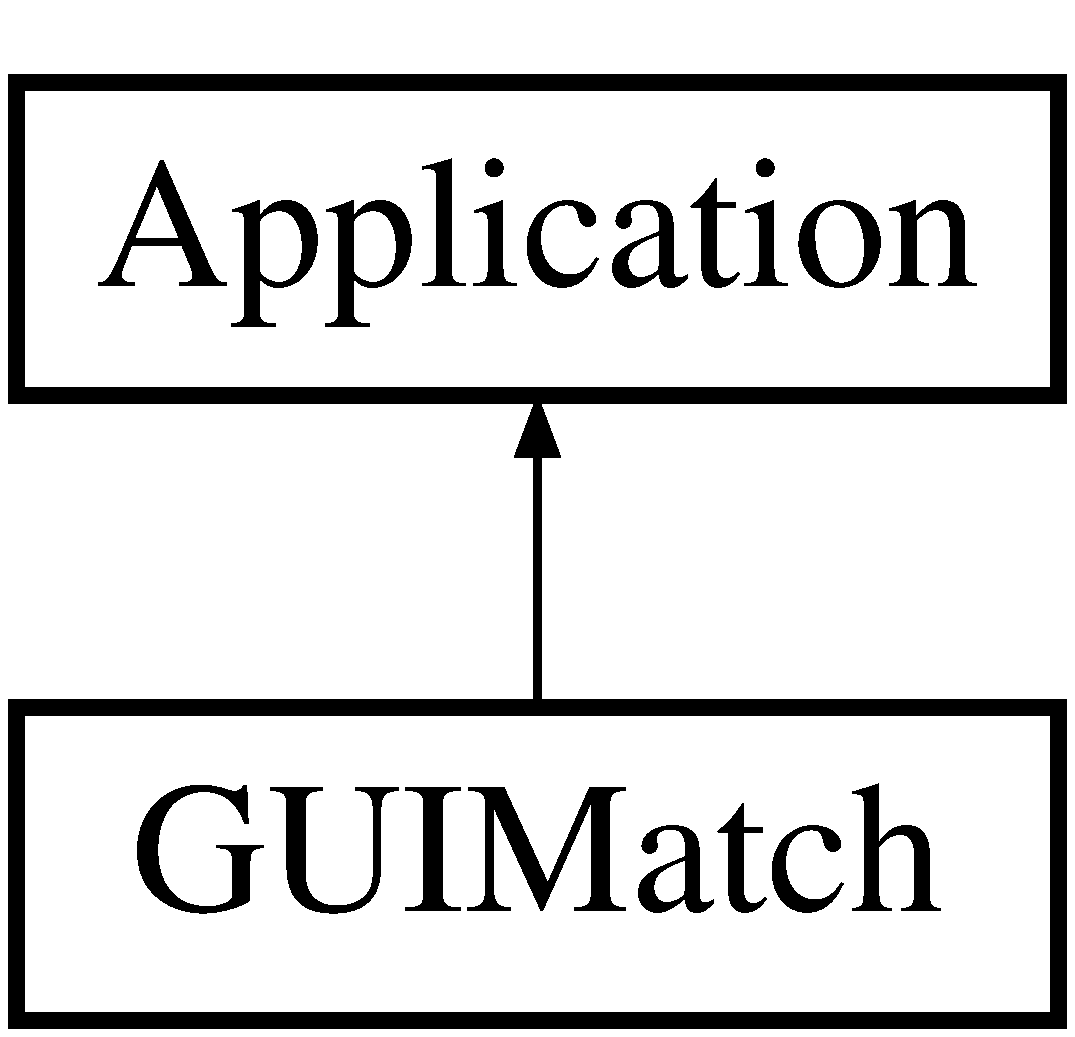
\includegraphics[height=2.000000cm]{class_g_u_i_match}
\end{center}
\end{figure}
\subsection*{Classes}
\begin{DoxyCompactItemize}
\item 
class \mbox{\hyperlink{class_g_u_i_match_1_1_my_key_handler}{My\+Key\+Handler}}
\end{DoxyCompactItemize}
\subsection*{Public Member Functions}
\begin{DoxyCompactItemize}
\item 
void \mbox{\hyperlink{class_g_u_i_match_a286efdec3789581a2892444cb193fe00}{start}} (Stage primary\+Stage)
\item 
void \mbox{\hyperlink{class_g_u_i_match_aa9f4fe916a6de3e9968e6eab465eb6e7}{set\+Up\+Pane}} (Stage primary\+Stage)
\end{DoxyCompactItemize}
\subsection*{Static Public Member Functions}
\begin{DoxyCompactItemize}
\item 
static void \mbox{\hyperlink{class_g_u_i_match_a76cccc2f3888f404094e9984d9fac3c8}{main}} (String\mbox{[}$\,$\mbox{]} args)
\end{DoxyCompactItemize}


\subsection{Member Function Documentation}
\mbox{\Hypertarget{class_g_u_i_match_a76cccc2f3888f404094e9984d9fac3c8}\label{class_g_u_i_match_a76cccc2f3888f404094e9984d9fac3c8}} 
\index{G\+U\+I\+Match@{G\+U\+I\+Match}!main@{main}}
\index{main@{main}!G\+U\+I\+Match@{G\+U\+I\+Match}}
\subsubsection{\texorpdfstring{main()}{main()}}
{\footnotesize\ttfamily static void G\+U\+I\+Match.\+main (\begin{DoxyParamCaption}\item[{String \mbox{[}$\,$\mbox{]}}]{args }\end{DoxyParamCaption})\hspace{0.3cm}{\ttfamily [static]}}

\mbox{\Hypertarget{class_g_u_i_match_aa9f4fe916a6de3e9968e6eab465eb6e7}\label{class_g_u_i_match_aa9f4fe916a6de3e9968e6eab465eb6e7}} 
\index{G\+U\+I\+Match@{G\+U\+I\+Match}!set\+Up\+Pane@{set\+Up\+Pane}}
\index{set\+Up\+Pane@{set\+Up\+Pane}!G\+U\+I\+Match@{G\+U\+I\+Match}}
\subsubsection{\texorpdfstring{set\+Up\+Pane()}{setUpPane()}}
{\footnotesize\ttfamily void G\+U\+I\+Match.\+set\+Up\+Pane (\begin{DoxyParamCaption}\item[{Stage}]{primary\+Stage }\end{DoxyParamCaption})}

\mbox{\Hypertarget{class_g_u_i_match_a286efdec3789581a2892444cb193fe00}\label{class_g_u_i_match_a286efdec3789581a2892444cb193fe00}} 
\index{G\+U\+I\+Match@{G\+U\+I\+Match}!start@{start}}
\index{start@{start}!G\+U\+I\+Match@{G\+U\+I\+Match}}
\subsubsection{\texorpdfstring{start()}{start()}}
{\footnotesize\ttfamily void G\+U\+I\+Match.\+start (\begin{DoxyParamCaption}\item[{Stage}]{primary\+Stage }\end{DoxyParamCaption})}



The documentation for this class was generated from the following file\+:\begin{DoxyCompactItemize}
\item 
\mbox{\hyperlink{_g_u_i_match_8java}{G\+U\+I\+Match.\+java}}\end{DoxyCompactItemize}

\hypertarget{class_match_grid}{}\section{Match\+Grid Class Reference}
\label{class_match_grid}\index{Match\+Grid@{Match\+Grid}}


The \mbox{\hyperlink{class_match_grid}{Match\+Grid}} class.  


\subsection*{Public Member Functions}
\begin{DoxyCompactItemize}
\item 
\mbox{\hyperlink{class_match_grid_acfd92ec568e826d6ea23fb7d2bb92800}{Match\+Grid}} ()
\begin{DoxyCompactList}\small\item\em The default constructor. \end{DoxyCompactList}\item 
int \mbox{\hyperlink{class_match_grid_a3ac68858317325bcd611aa811dab54ad}{get}} (int row, int col)
\begin{DoxyCompactList}\small\item\em A custom getter method. \end{DoxyCompactList}\item 
boolean \mbox{\hyperlink{class_match_grid_adc3b7a588c1b58a737f3ef45a10a7888}{show}} (int row, int col)
\begin{DoxyCompactList}\small\item\em A method that unhides the image and increases score if it matches. \end{DoxyCompactList}\item 
int \mbox{\hyperlink{class_match_grid_a39fcc7cc9b094d95d2aee459c9e287df}{get\+Score}} ()
\begin{DoxyCompactList}\small\item\em A method for getting the score. \end{DoxyCompactList}\item 
void \mbox{\hyperlink{class_match_grid_ada04481d2f01ef0011a7bb4707d2b911}{hide}} ()
\begin{DoxyCompactList}\small\item\em Hides all images. \end{DoxyCompactList}\item 
void \mbox{\hyperlink{class_match_grid_a67c79ef33744f135e5a9b483bf5e369f}{print\+Grid}} ()
\begin{DoxyCompactList}\small\item\em Prints the contents of grid\mbox{[}\mbox{]}\mbox{[}\mbox{]}. \end{DoxyCompactList}\end{DoxyCompactItemize}


\subsection{Detailed Description}
The \mbox{\hyperlink{class_match_grid}{Match\+Grid}} class. 

Sets up and populates the grid used for displaying the circles, and contains methods for interacting with it. 

\subsection{Constructor \& Destructor Documentation}
\mbox{\Hypertarget{class_match_grid_acfd92ec568e826d6ea23fb7d2bb92800}\label{class_match_grid_acfd92ec568e826d6ea23fb7d2bb92800}} 
\index{Match\+Grid@{Match\+Grid}!Match\+Grid@{Match\+Grid}}
\index{Match\+Grid@{Match\+Grid}!Match\+Grid@{Match\+Grid}}
\subsubsection{\texorpdfstring{Match\+Grid()}{MatchGrid()}}
{\footnotesize\ttfamily Match\+Grid.\+Match\+Grid (\begin{DoxyParamCaption}{ }\end{DoxyParamCaption})}



The default constructor. 

Populates the grid array with random values. $<$ The number of circles left to populate.

$<$ Used to select which circle will be populated. 

\subsection{Member Function Documentation}
\mbox{\Hypertarget{class_match_grid_a3ac68858317325bcd611aa811dab54ad}\label{class_match_grid_a3ac68858317325bcd611aa811dab54ad}} 
\index{Match\+Grid@{Match\+Grid}!get@{get}}
\index{get@{get}!Match\+Grid@{Match\+Grid}}
\subsubsection{\texorpdfstring{get()}{get()}}
{\footnotesize\ttfamily int Match\+Grid.\+get (\begin{DoxyParamCaption}\item[{int}]{row,  }\item[{int}]{col }\end{DoxyParamCaption})}



A custom getter method. 


\begin{DoxyParams}{Parameters}
{\em row} & the row to query \\
\hline
{\em col} & the column to query \\
\hline
\end{DoxyParams}
\begin{DoxyReturn}{Returns}
If it is showing, the grid index; if not, 0. 
\end{DoxyReturn}
\mbox{\Hypertarget{class_match_grid_a39fcc7cc9b094d95d2aee459c9e287df}\label{class_match_grid_a39fcc7cc9b094d95d2aee459c9e287df}} 
\index{Match\+Grid@{Match\+Grid}!get\+Score@{get\+Score}}
\index{get\+Score@{get\+Score}!Match\+Grid@{Match\+Grid}}
\subsubsection{\texorpdfstring{get\+Score()}{getScore()}}
{\footnotesize\ttfamily int Match\+Grid.\+get\+Score (\begin{DoxyParamCaption}{ }\end{DoxyParamCaption})}



A method for getting the score. 

\begin{DoxyReturn}{Returns}
The score of the game. 
\end{DoxyReturn}
\mbox{\Hypertarget{class_match_grid_ada04481d2f01ef0011a7bb4707d2b911}\label{class_match_grid_ada04481d2f01ef0011a7bb4707d2b911}} 
\index{Match\+Grid@{Match\+Grid}!hide@{hide}}
\index{hide@{hide}!Match\+Grid@{Match\+Grid}}
\subsubsection{\texorpdfstring{hide()}{hide()}}
{\footnotesize\ttfamily void Match\+Grid.\+hide (\begin{DoxyParamCaption}{ }\end{DoxyParamCaption})}



Hides all images. 

\mbox{\Hypertarget{class_match_grid_a67c79ef33744f135e5a9b483bf5e369f}\label{class_match_grid_a67c79ef33744f135e5a9b483bf5e369f}} 
\index{Match\+Grid@{Match\+Grid}!print\+Grid@{print\+Grid}}
\index{print\+Grid@{print\+Grid}!Match\+Grid@{Match\+Grid}}
\subsubsection{\texorpdfstring{print\+Grid()}{printGrid()}}
{\footnotesize\ttfamily void Match\+Grid.\+print\+Grid (\begin{DoxyParamCaption}{ }\end{DoxyParamCaption})}



Prints the contents of grid\mbox{[}\mbox{]}\mbox{[}\mbox{]}. 

\mbox{\Hypertarget{class_match_grid_adc3b7a588c1b58a737f3ef45a10a7888}\label{class_match_grid_adc3b7a588c1b58a737f3ef45a10a7888}} 
\index{Match\+Grid@{Match\+Grid}!show@{show}}
\index{show@{show}!Match\+Grid@{Match\+Grid}}
\subsubsection{\texorpdfstring{show()}{show()}}
{\footnotesize\ttfamily boolean Match\+Grid.\+show (\begin{DoxyParamCaption}\item[{int}]{row,  }\item[{int}]{col }\end{DoxyParamCaption})}



A method that unhides the image and increases score if it matches. 


\begin{DoxyParams}{Parameters}
{\em row} & the row to use \\
\hline
{\em col} & the column to use \\
\hline
\end{DoxyParams}
\begin{DoxyReturn}{Returns}
true if it completes, false if the image is already shown 
\end{DoxyReturn}


The documentation for this class was generated from the following file\+:\begin{DoxyCompactItemize}
\item 
\mbox{\hyperlink{_match_grid_8java}{Match\+Grid.\+java}}\end{DoxyCompactItemize}

\hypertarget{class_match_tile}{}\section{Match\+Tile Class Reference}
\label{class_match_tile}\index{Match\+Tile@{Match\+Tile}}
Inheritance diagram for Match\+Tile\+:\begin{figure}[H]
\begin{center}
\leavevmode
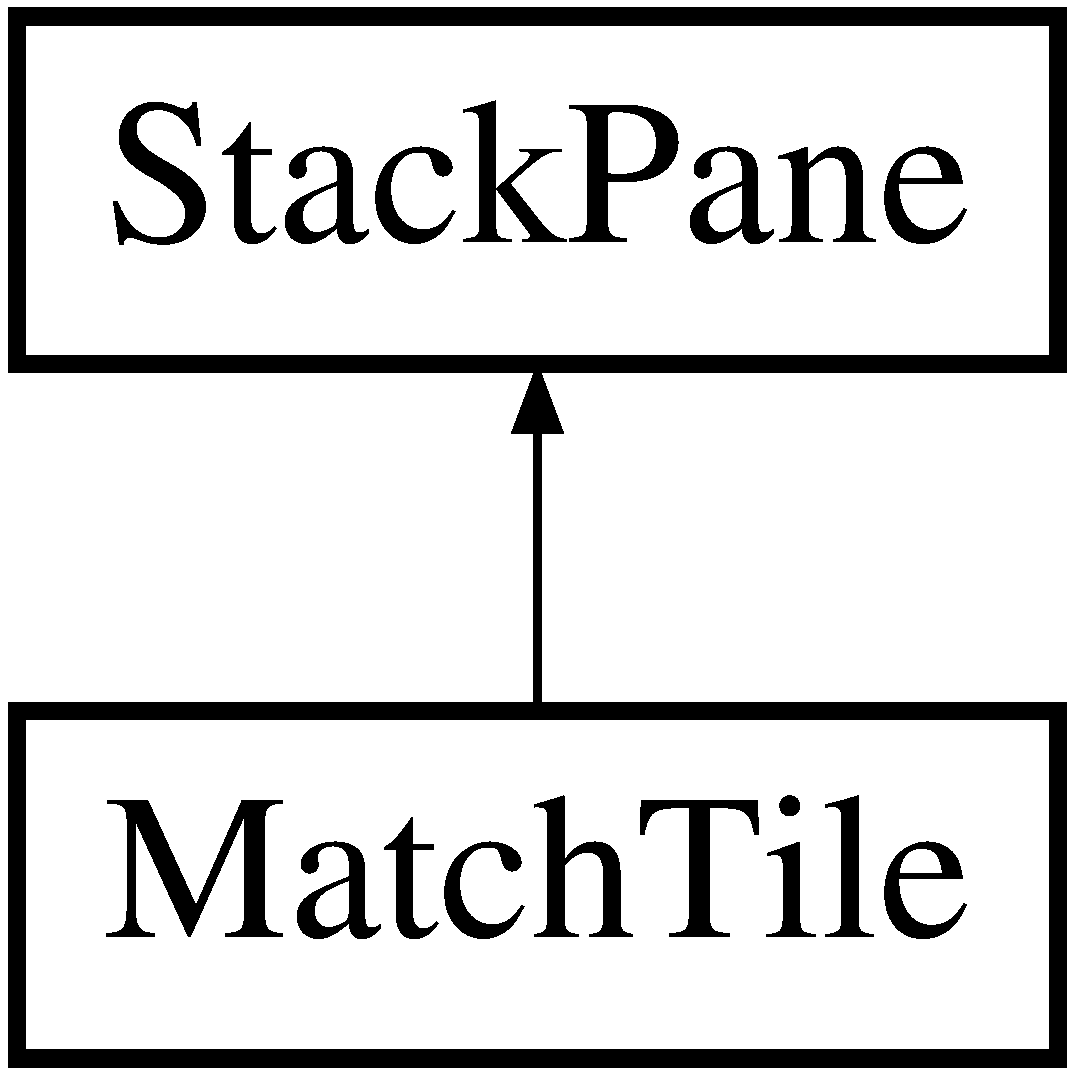
\includegraphics[height=2.000000cm]{class_match_tile}
\end{center}
\end{figure}
\subsection*{Public Member Functions}
\begin{DoxyCompactItemize}
\item 
\mbox{\hyperlink{class_match_tile_a273188eda4544581d4424e4681c33fb0}{Match\+Tile}} (int tile\+Value, int ro, int co)
\item 
int \mbox{\hyperlink{class_match_tile_a1524b5b7c525f3af9533cf8f83cacc13}{get\+Row}} ()
\item 
int \mbox{\hyperlink{class_match_tile_a76b318319525d1945da6402652c347b7}{get\+Col}} ()
\end{DoxyCompactItemize}
\subsection*{Static Public Member Functions}
\begin{DoxyCompactItemize}
\item 
static void \mbox{\hyperlink{class_match_tile_a0637f46e6d19de24cfe69181fe480284}{load\+Images}} ()
\end{DoxyCompactItemize}


\subsection{Constructor \& Destructor Documentation}
\mbox{\Hypertarget{class_match_tile_a273188eda4544581d4424e4681c33fb0}\label{class_match_tile_a273188eda4544581d4424e4681c33fb0}} 
\index{Match\+Tile@{Match\+Tile}!Match\+Tile@{Match\+Tile}}
\index{Match\+Tile@{Match\+Tile}!Match\+Tile@{Match\+Tile}}
\subsubsection{\texorpdfstring{Match\+Tile()}{MatchTile()}}
{\footnotesize\ttfamily Match\+Tile.\+Match\+Tile (\begin{DoxyParamCaption}\item[{int}]{tile\+Value,  }\item[{int}]{ro,  }\item[{int}]{co }\end{DoxyParamCaption})}



\subsection{Member Function Documentation}
\mbox{\Hypertarget{class_match_tile_a76b318319525d1945da6402652c347b7}\label{class_match_tile_a76b318319525d1945da6402652c347b7}} 
\index{Match\+Tile@{Match\+Tile}!get\+Col@{get\+Col}}
\index{get\+Col@{get\+Col}!Match\+Tile@{Match\+Tile}}
\subsubsection{\texorpdfstring{get\+Col()}{getCol()}}
{\footnotesize\ttfamily int Match\+Tile.\+get\+Col (\begin{DoxyParamCaption}{ }\end{DoxyParamCaption})}

\mbox{\Hypertarget{class_match_tile_a1524b5b7c525f3af9533cf8f83cacc13}\label{class_match_tile_a1524b5b7c525f3af9533cf8f83cacc13}} 
\index{Match\+Tile@{Match\+Tile}!get\+Row@{get\+Row}}
\index{get\+Row@{get\+Row}!Match\+Tile@{Match\+Tile}}
\subsubsection{\texorpdfstring{get\+Row()}{getRow()}}
{\footnotesize\ttfamily int Match\+Tile.\+get\+Row (\begin{DoxyParamCaption}{ }\end{DoxyParamCaption})}

\mbox{\Hypertarget{class_match_tile_a0637f46e6d19de24cfe69181fe480284}\label{class_match_tile_a0637f46e6d19de24cfe69181fe480284}} 
\index{Match\+Tile@{Match\+Tile}!load\+Images@{load\+Images}}
\index{load\+Images@{load\+Images}!Match\+Tile@{Match\+Tile}}
\subsubsection{\texorpdfstring{load\+Images()}{loadImages()}}
{\footnotesize\ttfamily static void Match\+Tile.\+load\+Images (\begin{DoxyParamCaption}{ }\end{DoxyParamCaption})\hspace{0.3cm}{\ttfamily [static]}}



The documentation for this class was generated from the following file\+:\begin{DoxyCompactItemize}
\item 
\mbox{\hyperlink{_match_tile_8java}{Match\+Tile.\+java}}\end{DoxyCompactItemize}

\hypertarget{class_g_u_i_match_1_1_my_key_handler}{}\section{G\+U\+I\+Match.\+My\+Key\+Handler Class Reference}
\label{class_g_u_i_match_1_1_my_key_handler}\index{G\+U\+I\+Match.\+My\+Key\+Handler@{G\+U\+I\+Match.\+My\+Key\+Handler}}
Inheritance diagram for G\+U\+I\+Match.\+My\+Key\+Handler\+:\begin{figure}[H]
\begin{center}
\leavevmode
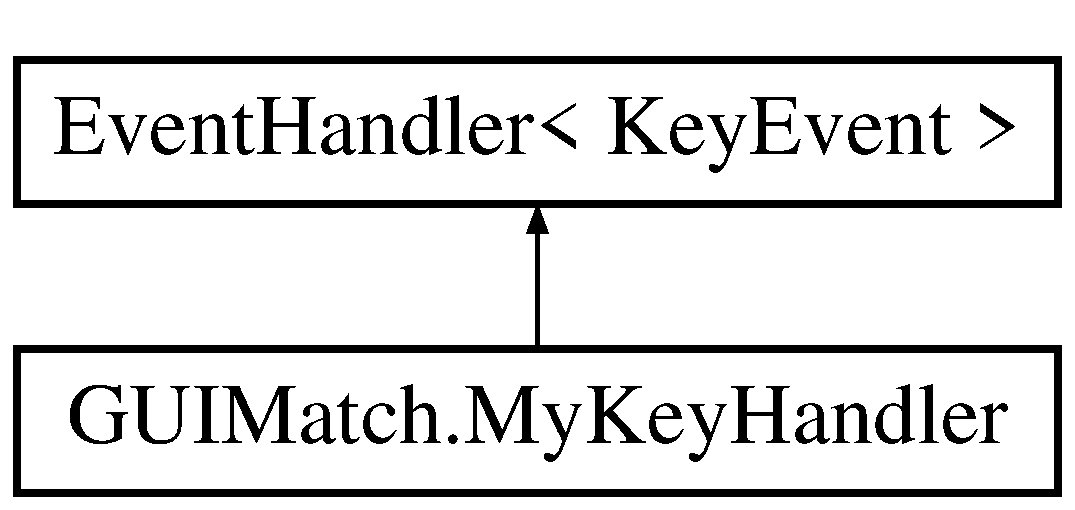
\includegraphics[height=2.000000cm]{class_g_u_i_match_1_1_my_key_handler}
\end{center}
\end{figure}
\subsection*{Public Member Functions}
\begin{DoxyCompactItemize}
\item 
void \mbox{\hyperlink{class_g_u_i_match_1_1_my_key_handler_a7ffde9d66d488a8de77f30238154e82c}{handle}} (Key\+Event e)
\end{DoxyCompactItemize}


\subsection{Member Function Documentation}
\mbox{\Hypertarget{class_g_u_i_match_1_1_my_key_handler_a7ffde9d66d488a8de77f30238154e82c}\label{class_g_u_i_match_1_1_my_key_handler_a7ffde9d66d488a8de77f30238154e82c}} 
\index{G\+U\+I\+Match\+::\+My\+Key\+Handler@{G\+U\+I\+Match\+::\+My\+Key\+Handler}!handle@{handle}}
\index{handle@{handle}!G\+U\+I\+Match\+::\+My\+Key\+Handler@{G\+U\+I\+Match\+::\+My\+Key\+Handler}}
\subsubsection{\texorpdfstring{handle()}{handle()}}
{\footnotesize\ttfamily void G\+U\+I\+Match.\+My\+Key\+Handler.\+handle (\begin{DoxyParamCaption}\item[{Key\+Event}]{e }\end{DoxyParamCaption})}



The documentation for this class was generated from the following file\+:\begin{DoxyCompactItemize}
\item 
\mbox{\hyperlink{_g_u_i_match_8java}{G\+U\+I\+Match.\+java}}\end{DoxyCompactItemize}

\chapter{File Documentation}
\hypertarget{_g_u_i_match_8java}{}\section{G\+U\+I\+Match.\+java File Reference}
\label{_g_u_i_match_8java}\index{G\+U\+I\+Match.\+java@{G\+U\+I\+Match.\+java}}
\subsection*{Classes}
\begin{DoxyCompactItemize}
\item 
class \mbox{\hyperlink{class_g_u_i_match}{G\+U\+I\+Match}}
\item 
class \mbox{\hyperlink{class_g_u_i_match_1_1_my_key_handler}{G\+U\+I\+Match.\+My\+Key\+Handler}}
\end{DoxyCompactItemize}

\hypertarget{_match_grid_8java}{}\section{Match\+Grid.\+java File Reference}
\label{_match_grid_8java}\index{Match\+Grid.\+java@{Match\+Grid.\+java}}
\subsection*{Classes}
\begin{DoxyCompactItemize}
\item 
class \mbox{\hyperlink{class_match_grid}{Match\+Grid}}
\begin{DoxyCompactList}\small\item\em The \mbox{\hyperlink{class_match_grid}{Match\+Grid}} class. \end{DoxyCompactList}\end{DoxyCompactItemize}

\hypertarget{_match_tile_8java}{}\section{Match\+Tile.\+java File Reference}
\label{_match_tile_8java}\index{Match\+Tile.\+java@{Match\+Tile.\+java}}
\subsection*{Classes}
\begin{DoxyCompactItemize}
\item 
class \mbox{\hyperlink{class_match_tile}{Match\+Tile}}
\end{DoxyCompactItemize}

%--- End generated contents ---

% Index
\backmatter
\newpage
\phantomsection
\clearemptydoublepage
\addcontentsline{toc}{chapter}{Index}
\printindex

\end{document}
